\section{Proceso de pentesting} 

\subsection{¿Que es un prueba de penetración o pentest?}
Según la definición de OWASP \cite{web1} un test de penetración o pentesting, a veces denominado 
prueba de caja negra, es esencialmente el arte de probar
un sistema o aplicación para descubrir vulnerabilidades de seguridad, sin conocer el funcionamiento interno de la mismas. Normalmente el equipo 
encargado de las pruebas de penetración accede a las aplicaciones como si fuesen usuarios. El pentester tratará con 
que ese nivel de acceso encontrar vulnerabilidades que se puedan explotar en la aplicación.

El propósito de la prueba de penetración es determinar la presencia 
de vulnerabilidades potencialmente explotables y analizar el impacto de estas,
sí se detecta alguna. La mejor forma de probar una defensa es tratando de penetrar en ella.
\clearpage
\newpage

\subsection{Fases del prueba de intrusión}
A la hora de realizar una prueba de intrusión o pentest distinguimos las siguientes fases, basándonos en 
la distinción realizada en pentesting con Kali  \cite{ref1};  dicjhas fases son las siguientes:
\begin{itemize}
    \item Alcance y términos de la prueba de intrusión.
    \item Recolección de información.
    \item Análisis de vulnerabilidades.
    \item Explotación de vulnerabilidades.
    \item Postexplotación del sistema.
    \item Generación de informes.
\end{itemize}
\subsubsection{Alcance y términos de la prueba de intrusión.}  
Para esta fase normalmente se genera un documento de plan de pruebas. En muchos casos es 
necesaria la revisión y aprobación de dicho documento por parte del dueño del sistema a probar 
(\gls{sut}), antes de poder comenzar con el proceso de pentesting.
    En dicho documento de pruebas se suel detallar la siguiente información:
    \begin{itemize}
        \item Sistema sobre el que se realizan las pruebas.
        \item Los tipos de prueba a realizar.
        \item Herramientas que se van a utilizar.
        \item Proceso de seguimiento de los defectos encontrados.
        \item Documentos que se entregarán durante el proceso de pentesting.
        \item Restricciones en la ejecución de la prueba de intrusión
    \end{itemize}

\subsubsection{Recolección de información.}
Una vez definido el plan de pruebas procederemos a recolectar información 
del sistema o aplicación indicado en dicho plan. 
        
Principalmente obtendremos información mediante los procesos de enumeración y 
análisis de código que detallaremos en el siguiente capítulo. 

\subsubsection{Análisis de vulnerabilidades.}
Al finalizar los procesos anteriores se analizarán los defectos encontrados para descartar falsos positivos y 
después se hará entrega un reporte de análisis dinámico con los defectos no descartados. 
Para cada uno de los defectos detectados que se incluyan en el reporte abriremos defecto en el sistema de gestión de defectos.

\subsubsection{Explotación de vulnerabilidades.}

En el caso de que uno o varios defectos necesiten ser explotados, y siempre solicitando permiso se detallará 
el proceso de explotación indicando las herramientas y \glspl{exploit} necesarios para realizar este proceso. 
En este proceso también se deben detallar las consecuencias, si las hubiese de la ejecución de las herramientas y 
exploits a utilizar sobre la aplicación o sistema objetivo.

\subsubsection{Postexplotación del sistema.}

En este caso también es necesario solicitar permiso al dueño del sistema, detallando 
la forma en que persistirá el ataque en la aplicación o sistema objetivo.

\subsubsection{Generación de informes.}

Llegados a este punto ya se deben haber hecho entrega de los reportes del análisis estático, si se dispone de acceso al código fuente, y del reporte de análisis dinámico. Sí se ejecutasen los procesos de explotación o Postexplotación se ampliaría el reporte de análisis dinámico con la información recabada en dichos procesos.

A parte de los reportes anteriores, se debe entregar un informe de resultado de 
pruebas con el resultado de ejecución del proceso de pentest incluyendo en 
el mismo el detalle de los defectos reportados en el sistema de gestión de 
defectos, si es posible, así como el estado en que se encuentran en el momento
de entrega de dicho reporte.

\clearpage
\newpage

\section{Detalle y Clasificación de vulnerabilidades OWASP Top 10}

El proceso de enumeración trataremos de recabar información de recurso accesibles del sistema 
o aplicación. Para este proceso existen númerosas utilidades, entre las más utilizadas estarían:

En índice de vulnerabilidades web OWASP Top 10, \href{https://wiki.owasp.org/images/5/5e/OWASP-Top-10-2017-es.pdf}{versión 2017}, 
clasifica los vulnerabilidades más comunes encontradas en los datos de aportados por cientos de organizaciones 
y más de 100.000 aplicaciones y servicios web del mundo real.

En su última versión las vulnerabilidades más comunes encontradas fueron las siguientes:

\begin{figure}[!htb] 
    \centering
    \captionsetup{width=1\linewidth} 
    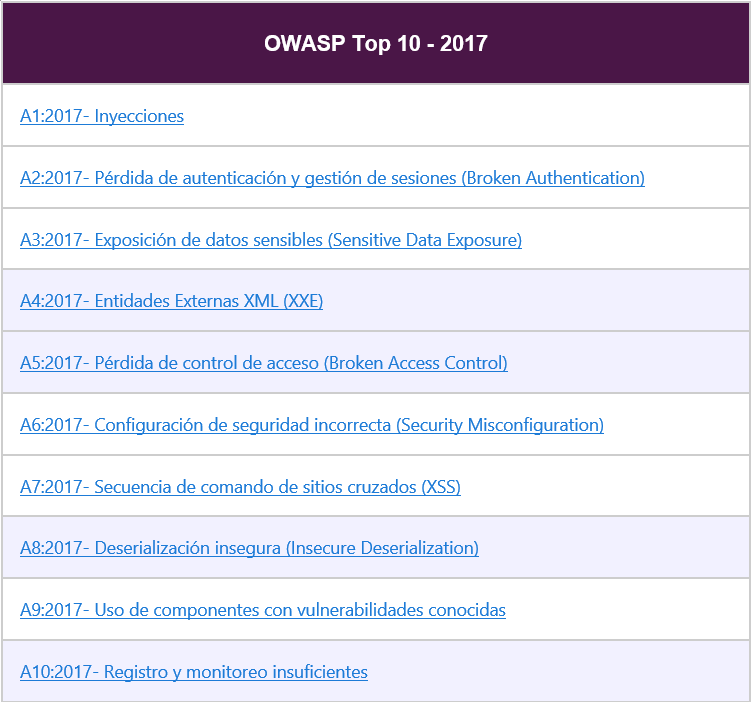
\includegraphics[width=\linewidth]{./imagenes/012_OWASP_Top_10_2017.png}
    \caption{OWASP Top 10 2017.}  
\end{figure}

A continuación, detallamos en qué consisten cada una de las vulnerabilidades listadas en el OWASP top 10:

\subsection{A1:2017 - Inyecciones}

Las fallas de inyección, como SQL, NoSQL, comandos o LDAP ocurren cuando se envían datos no
confiables a un intérprete, como parte de un comando o consulta. Los datos dañinos del atacante
pueden engañar al intérprete para que ejecute comandos involuntarios o acceda a los datos sin
la debida autorización.

La inyección de SQL (SQLi) es uno de los tipos de ataques de inyección de código más
comunes y peligrosos, aprovechados por los atacantes con la intención de obtener
información no autorizada o en sí generar problemas en los servidores de base de datos y
comportamiento de aplicaciones.

Por Ejemplo, en la siguiente aplicación tenemos un formulario para mostrar 
la información de un usuario a partir de su identificador (ID):

\begin{figure}[!htb]  
    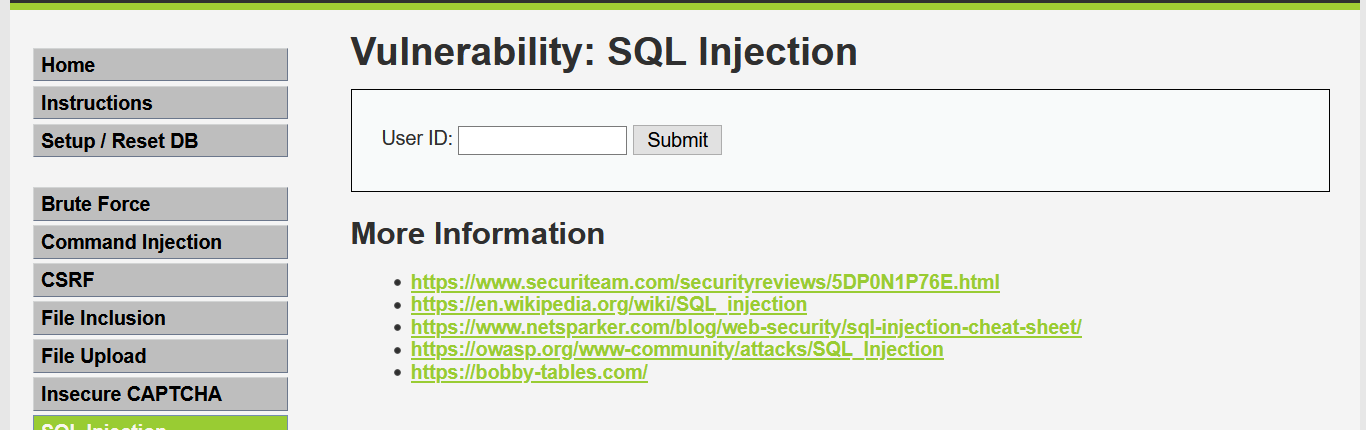
\includegraphics[width=\linewidth]{./imagenes/013_SQLi_Example_1.png}
    \caption{Aplicación vulnerable SQLi.}  
\end{figure}

Un uso normal generaría este tipo de peticiones:

\begin{figure}[!htb]  
    \centering
    \captionsetup{width=1\linewidth}
    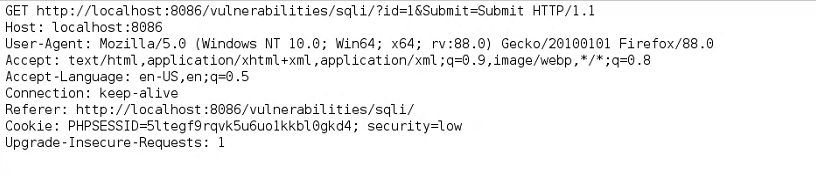
\includegraphics[width=\linewidth]{./imagenes/013_SQLi_Example_2.png}
    \caption{Petición normal}  
\end{figure}

\newpage
Pero si abusamos de la aplicación modificando el ID por la consulta:\\
\begin{verbatim}
    %' union select user,password from users# 
\end{verbatim}

Se genera la siguiente petición:\\
\begin{figure}[!htb]
    \centering
    \captionsetup{width=1\linewidth}  
    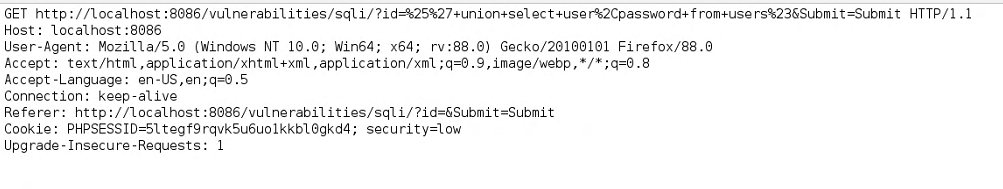
\includegraphics[width=\linewidth]{./imagenes/013_SQLi_Example_3.png}
    \caption{Ejemplo Ataque SQLi.}  
    \label{fig:4 - SQLi 3}
\end{figure}

El resultado será que la aplicación nos devuelve todos los usuarios y password almacenados en la Base de datos:\\
\begin{figure}[!htb]  
    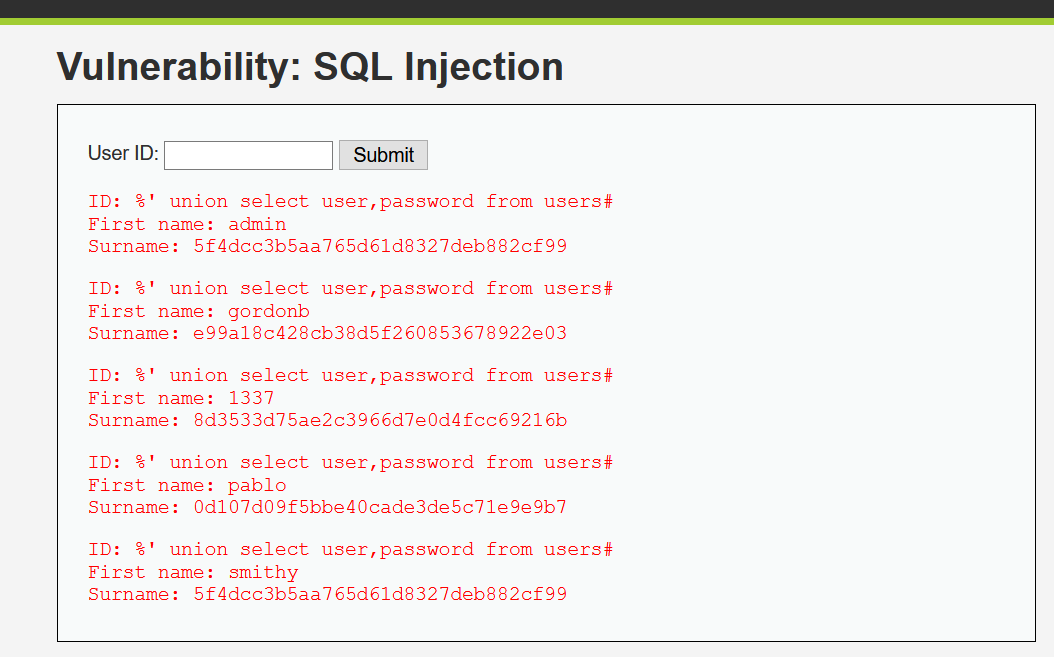
\includegraphics[width=\linewidth]{./imagenes/013_SQLi_Example_4.png}
    \caption{Resultado ataque SQLi.}  
    \label{fig:5 - SQLi 3}
\end{figure}

\newpage
\subsection{A2:2017 - Pérdida de autenticación y gestión de sesiones (Broken Authentication)}

Las funciones de la aplicación relacionadas a autenticación y gestión de sesiones son
implementadas incorrectamente, permitiendo a los atacantes comprometer usuarios y
contraseñas, token de sesiones, o explotar otras fallas de implementación para asumir la
identidad de otros usuarios (temporal o permanentemente).

En los últimos años se han detectado numerosas aplicaciones, sobre todo la que hacen uso de api para 
la gestión de los datos, que hacen uso de JSON Web Tokens (JWT) para la autenticación y autorización. 

\begin{figure}[!htb]  
    \centering
    \captionsetup{width=1\linewidth}  
    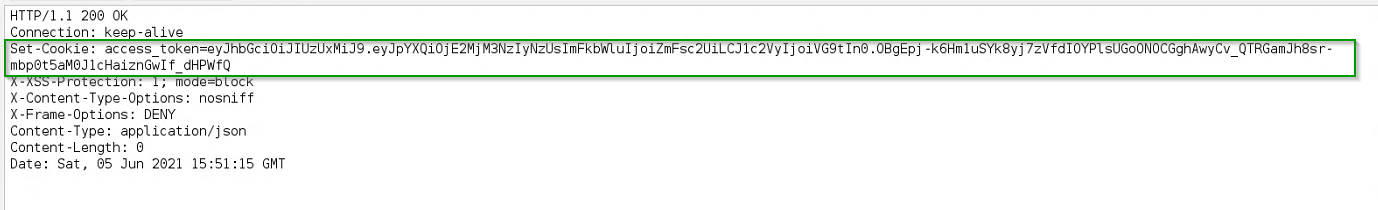
\includegraphics[width=\linewidth]{./imagenes/014_BrokenAuthentication_1.png}
    \caption{Token JWT.}  
    \label{fig:Token JWT}
\end{figure}

La captura de este token permite a los atacantes a realizar peticiones en nombre del usuario, puesto que, 
si decodificamos el token, podemos ver que identifica a un usuario concreto

\begin{figure}[!htb]
    \centering
    \captionsetup{width=1\linewidth}    
    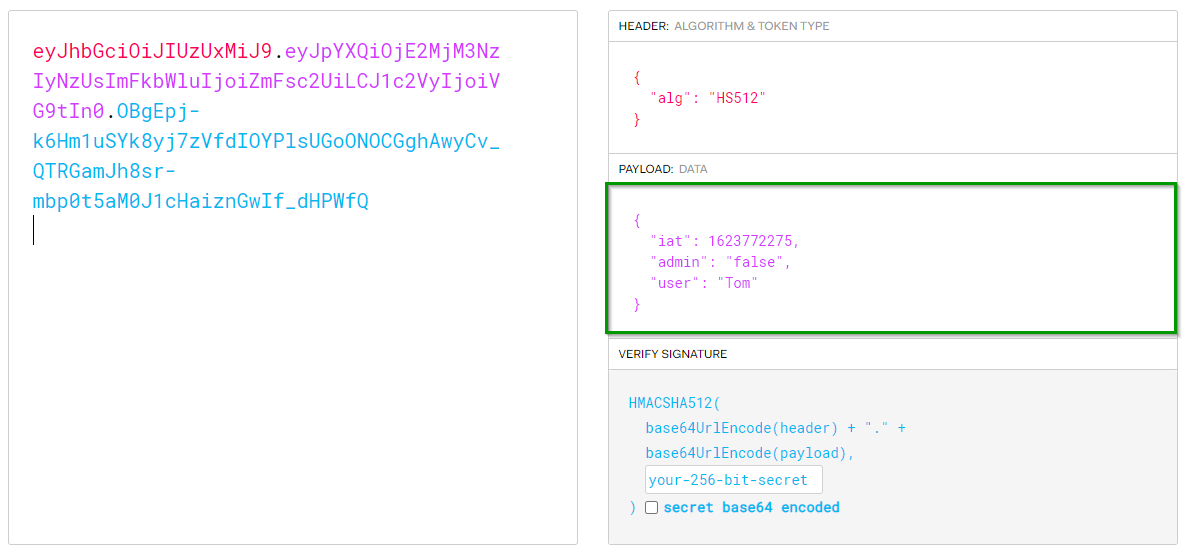
\includegraphics[width=\linewidth]{./imagenes/014_BrokenAuthentication_2.png}
    \caption{Token JWT decodificado.}  
    \label{fig:Token JWT decodificado}
\end{figure}

\newpage
Lo cual nos permite realizar cualquier petición en nombre del usuario haciendo uso de su token JWT.

\begin{figure}[!htb] 
    \centering
    \captionsetup{width=1\linewidth}   
    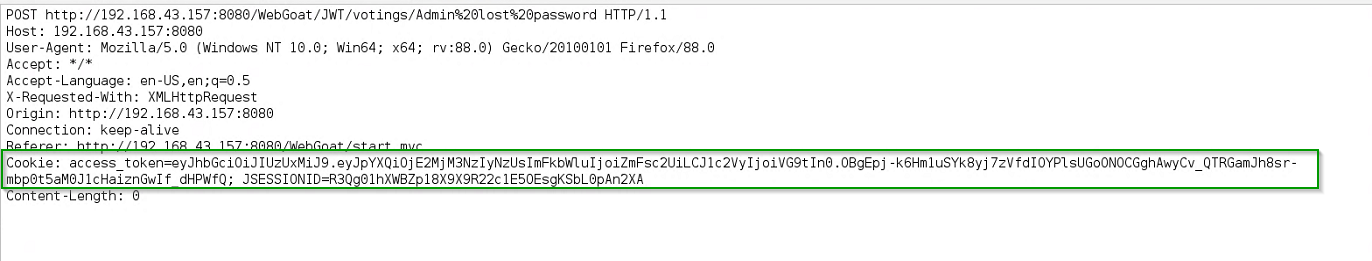
\includegraphics[width=\linewidth]{./imagenes/014_BrokenAuthentication_3.png}
    \caption{Ataque Broken Authentication.}  
    \label{fig:Broken Authentication attack}
\end{figure}

\subsection{A3:2017 - Exposición de datos sensibles (Sensitive Data Exposure)}

Muchas aplicaciones y servicios web no protegen adecuadamente datos sensibles, tales como
información financiera, de salud o Información Personalmente Identificable (PII). Los atacantes
pueden robar o modificar estos datos protegidos inadecuadamente para llevar a cabo fraudes
con tarjetas de crédito, robos de identidad u otros delitos. Los datos sensibles requieren métodos
de protección adicionales, como el cifrado en almacenamiento y tránsito. 

\subsection{A4:2017 - XML External Entities (XXE)}

Muchos procesadores XML antiguos o mal configurados evalúan referencias a entidades externas en 
documentos XML. Las entidades externas pueden utilizarse para revelar archivos internos mediante la URI 
o archivos internos en servidores no actualizados, escanear puertos de la LAN, ejecutar código de forma
 remota y realizar ataques de denegación de servicio (DoS).

Una entidad XML permite definir etiquetas que serán reemplazadas por contenido cuando se analice 
el documento XML. En general, existen tres tipos de entidades: 

\begin{itemize}
    \item Entidades internas.
    \item Entidades externas.
    \item Entidades parametrizadas.
\end{itemize}

Una entidad debe ser definida en el “Document Type Definition” (DTD), vemos un ejemplo:

\begin{listing}[!htb]
    \inputminted{xml}{./Ficheros/DTD_example.xml}
    \caption{DTD example}
    \label{listing:1}
\end{listing}

En este caso el \gls{parser} de XML carga la entidad externa \textbf{"SYSTEM"} que obtendrá el contenido del 
fichero \textbf{"/etc/passwd"} y devolverá el contenido de este fichero en la respuesta:

\begin{figure}[!htb]  
    \centering
    \captionsetup{width=1\linewidth}  
    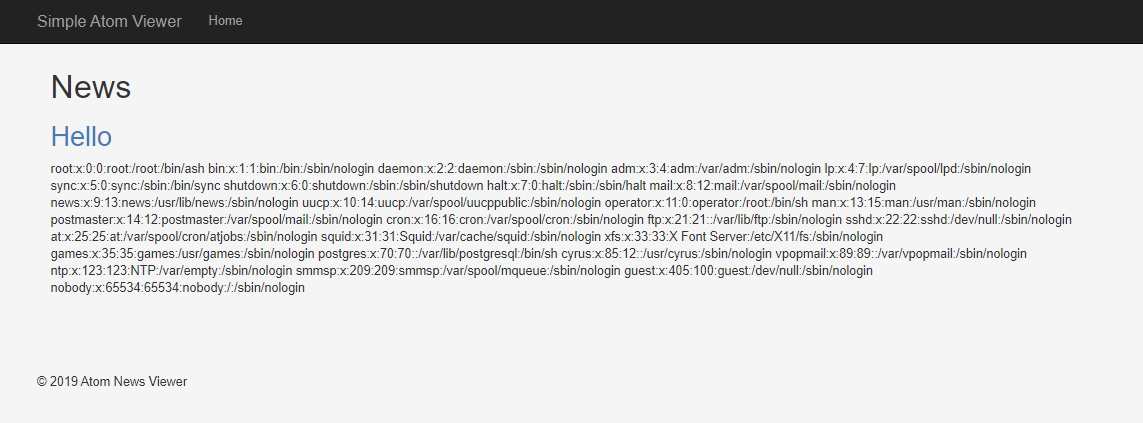
\includegraphics[width=\linewidth]{./imagenes/015_XXE_Attack_1.png}
    \caption{Ataque XXE.}  
    \label{fig:6 - XXE attack}
\end{figure}

Por lo tanto, un ataque de entidad externa XML es un tipo de ataque contra una aplicación que analiza 
la entrada XML. Este ataque ocurre cuando la entrada XML que contiene una referencia a una 
entidad externa es procesada por un analizador XML configurado débilmente. 

Este ataque puede conducir a la divulgación de datos confidenciales, denegación de servicio, falsificación 
de solicitudes del lado del servidor, escaneo de puertos desde la perspectiva de la máquina donde se 
encuentra el analizador y otros impactos del sistema.

\newpage
\subsection{A5:2017 - Pérdida de control de acceso (Broken Access Control)}

Las restricciones sobre lo que los usuarios autenticados pueden hacer no se aplican
correctamente. Los atacantes pueden explotar estos defectos para acceder, de forma no
autorizada, a funcionalidades y/o datos, cuentas de otros usuarios, ver archivos sensibles,
modificar datos, cambiar derechos de acceso y permisos, etc. 

\subsection{A6:2017 - Configuración de seguridad incorrecta (Security Misconfiguration)}

La configuración de seguridad incorrecta es un problema muy común y se debe en parte a
establecer la configuración de forma manual, ad hoc o por omisión (o directamente por la falta de
configuración). 

Son ejemplos: S3 buckets abiertos, cabeceras HTTP mal configuradas, mensajes
de error con contenido sensible, falta de parches y actualizaciones, frameworks, dependencias y
componentes desactualizados, etc.

\subsection{A7:2017 - Secuencia de comando de sitios cruzados (XSS)}

Los XSS ocurren cuando una aplicación toma datos no confiables y los envía al navegador web
sin una validación y codificación apropiada; o actualiza una página web existente con datos
suministrados por el usuario utilizando una API que ejecuta JavaScript en el navegador.

Permiten ejecutar comandos en el navegador de la víctima y el atacante puede secuestrar una sesión, modificar (\gls{defacement}) los sitios web, o redireccionar al usuario hacia un sitio malicioso.

Por ejemplo, si tenemos una aplicación como la siguiente con un formulario de entrada de datos como el siguiente:

\begin{figure}[!htb]  
    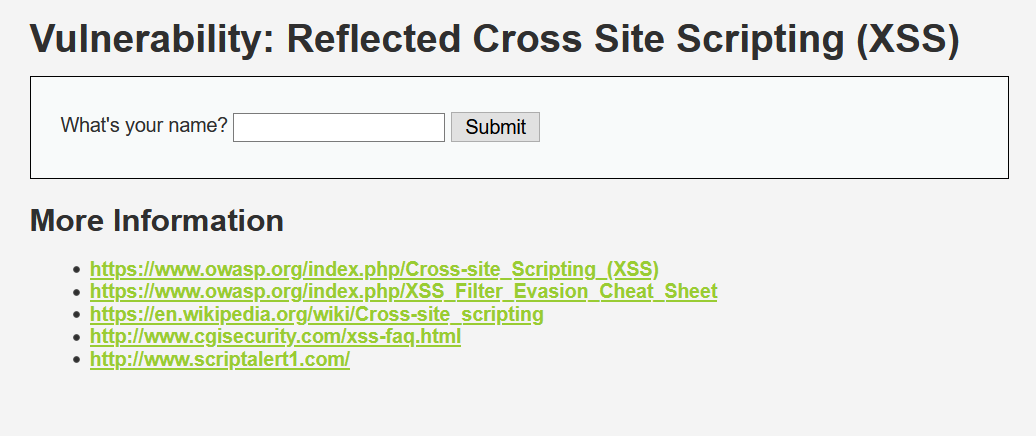
\includegraphics[width=\linewidth]{./imagenes/016_XSS_1.png}
    \caption{Aplicacion insegura XXS.}  
    \label{fig:7 - Aplicacion insegura XXS.}
\end{figure}

Si introducimos el siguiente script:

\begin{verbatim}
    <script>alert(document.cookie)</script>
\end{verbatim}

Vemos que al enviar el formulario se ejecuta el script en el navegador.\\

\begin{figure}[!htb] 
    \centering
    \captionsetup{width=1\linewidth}   
    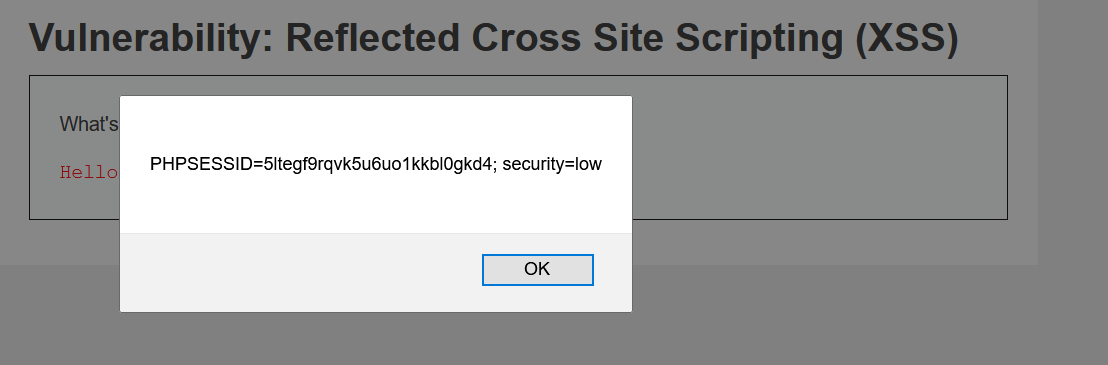
\includegraphics[width=\linewidth]{./imagenes/016_XSS_2.png}
    \caption{Ataque XXS.}  
    \label{fig:8 - Ataque XXS.}
\end{figure}

Podemos distinguir tres tipos de ataques XSS:\\
\begin{itemize}
    \item \textbf{Reflejados:} Cuando el script malicioso está presente en la petición HTTP.
    \item \textbf{Almacenados:} El script malicioso es almacenado en el servidor, en la base 
    de datos, en un fichero del sistema o cualquier otor objeto, y es visible cuando se muestra 
    la página en el navegador.
    \item \textbf{Basados en el DOM:} Técnicamente se consideraría reflejado. Ocurre cuando el script 
    malicioso incluye código html en la petición HTTP.
\end{itemize}

\newpage
\subsection{A8:2017 - Deserialización insegura (Insecure Deserialization) }

Estos defectos ocurren cuando una aplicación recibe objetos serializados dañinos y estos objetos
pueden ser manipulados o borrados por el atacante para realizar ataques de repetición,
inyecciones o elevar sus privilegios de ejecución. En el peor de los casos, la deserialización
insegura puede conducir a la ejecución remota de código en el servidor. 

La serialización es el proceso de convertir un objeto en un formato de datos que se puede restaurar 
más tarde. Las personas a menudo serializan objetos para guardarlos en el almacenamiento o para enviarlos 
como parte de las comunicaciones. La deserialización es lo contrario de ese proceso que toma datos
estructurados de algún formato y los reconstruye en un objeto.

Hoy en día, el formato de datos más popular para serializar datos es JSON, no hace mucho el 
formato más común era XML.

Muchos lenguajes de programación ofrecen una capacidad nativa para serializar objetos. Estos formatos 
nativos suelen ofrecer más funciones que JSON o XML, incluida la personalización del proceso de 
serialización. Desafortunadamente, las características de estos mecanismos de deserialización 
nativos pueden reutilizarse para generar efectos maliciosos cuando se opera con datos que no son de confianza.

Se ha descubierto que los ataques de deserialización permiten ataques de denegación de servicio, control 
de acceso y ejecución remota de código. Los lenguajes de programación que se han conocido ataques de este 
tipo serian:

\begin{itemize}
    \item PHP
    \item Python
    \item Ruby
    \item Java
    \item C$\backslash$C++
\end{itemize}

Por ejemplo, este código Java aprovecha la serialización para codificar una tarea que detenga 
la aplicación durante 5 segundos:

\begin{listing}[!htb]
    \inputminted{java}{./Ficheros/Serialize.java}
    \caption{Java Serialize Code}
    \label{listing:2}
\end{listing}

Este código crea la tarea y la serializa generando el siguiente token:

\begin{verbatim}
    rO0ABXNyADFvcmcuZHVtbXkuaW5zZWN1cmUuZnJhbWV3b3JrLlZ1bG5lcmFibGVUYXNrSG9sZGV
    yAAAAAAAAAAICAANMABZyZXF1ZXN0ZWRFeGVjdXRpb25UaW1ldAAZTGphdmEvdGltZS9Mb2NhbE
    RhdGVUaW1lO0wACnRhc2tBY3Rpb250ABJMamF2YS9sYW5nL1N0cmluZztMAAh0YXNrTmFtZXEAf
    gACeHBzcgANamF2YS50aW1lLlNlcpVdhLobIkiyDAAAeHB3DgUAAAflBgYSCgML+WfAeHQAB3Ns
    ZWVwIDV0AAZteVRhc2s=
\end{verbatim}

Dicho token al ser enviado en una petición al servidor provoca que la aplicación se detenga durante 5 segundos.

\newpage
\subsection{A9:2017 - Uso de componentes con vulnerabilidades conocidas}

Los componentes como bibliotecas, frameworks y otros módulos se ejecutan con los mismos
privilegios que la aplicación. Si se explota un componente vulnerable, el ataque puede provocar
una pérdida de datos o tomar el control del servidor. Las aplicaciones y API que utilizan
componentes con vulnerabilidades conocidas pueden debilitar las defensas de las aplicaciones y
permitir diversos ataques e impactos.

\subsection{2.2.10. A10:2017 - Registro y monitoreo insuficientes}

El registro y monitoreo insuficiente, junto a la falta de respuesta ante incidentes permiten a los
atacantes mantener el ataque en el tiempo, pivotear a otros sistemas y manipular, extraer o
destruir datos. Los estudios muestran que el tiempo de detección de una brecha de seguridad es
mayor a 200 días, siendo típicamente detectado por terceros en lugar de por procesos internos. 


\newpage



\section{Herramientas de análisis de código}

Detro de los procesos actuales de \gls{ssdlc} cada vez cobran más importacia la inclusion de herramientas de analisis de codigo durante el proceso de desarrollo del Software.

Dentro de las herramientas de análisis de código, podemos hacer la siguietne distinción:

\begin{itemize}
    \item \textbf{Herramientas de Análisis de código estático (\Gls{sast}).} 
    El análisis estático es un proceso que se realiza sobre el código de una aplicación 
    sin necesidad de ejecutarse.

    El  análisis de código estático, también conocido como Análisis de código fuente \Gls{sca}, 
    realiza pruebas sobre el código fuente para la detección temprana de defectos en dicho código. El uso de este
    tipo de herramientas es recomendable realizarlos en la fase de implementación del ciclo
    de desarrollo seguro  \gls{ssdlc}.

    \item \textbf{Herramientas de análisis de código Dinámico (\Gls{dast}.)} 
    Este tipo de análisis se realiza sobre una aplicación o servicio desplegado y en ejecución, a diferencia del tipo anterior.

    En análisis DAST enviará peticiones maliciosas al sistema objetivo para verificar la presencia de diversos tipos de ataques.

        
    \item \textbf{Herramientas híbridas.} 
    Las herramientas hibridas son aquellas que presentan proceso para definir los dos tipos de análisis anteriores.
\end{itemize}
    

\subsection{Herramientas de análisis estático de código}

La metodología  \gls{owasp} \gls{asvs} 4.0 se introdujo una sección para añadir 
los controles de codigo fuente como un requisito más dentro 
de la lista de requerimientos  para un desarrollo seguro:

\begin{figure}[h!]  
    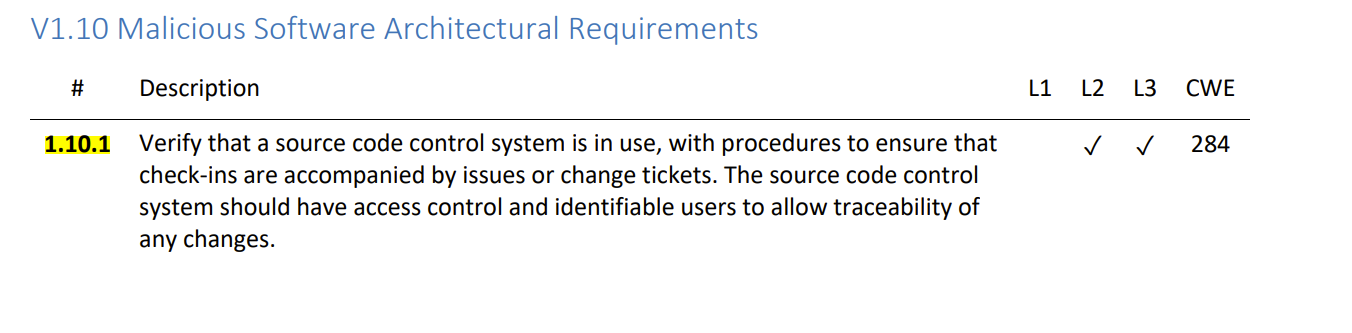
\includegraphics[width=\linewidth]{./imagenes/01_OWASP Application Security Verification Standard 4.0.png}
    \caption{ASVS 4.0 10.0.1 Security control.}  
\end{figure}

Actualmete en mucho de los ciclos de desarrollo estas herramientas se encuentran integradas dentro de los procesos de Integración 
continua (\gls{ci}) y despliegue continuo (\gls{cd}), esto permite que ante cualquier cambio en el código se ejecuten estas
herramientas de forma automática permitiendo que ante cualquier cambio se ejecuten este tipo de herramientas de forma 
automática en los procesos de compilación y despliegue. 

También es común que las herramientas de análisis de código estén integradas dentro de los IDEs de desarrollo; lo cual permite 
que los desarrolladores también puedan hacer uso de estas herramientas y mejorar la calidad del código antes de su entrega.

Entre las distintas herramientas de análisis, para la implementación de nuestra infraestructura de pruebas haremos uso 
de las siguientes herramientas:
\begin{itemize}
    \item SonarQube
    \item Dependency-check
\end{itemize}
\newpage

\subsubsection{SonarQube}
Es una plataforma de para el análisis estático de código, dispone de distintos escáneres para la mayor parte de 
lenguajes de programación. Entre las versiones disponibles de SonarQube, podemos hacer uso de la 
versión \emph{“Community”} que es de uso libre.

\begin{figure}[!htb]
    \centering
    \captionsetup{width=1\linewidth}     
    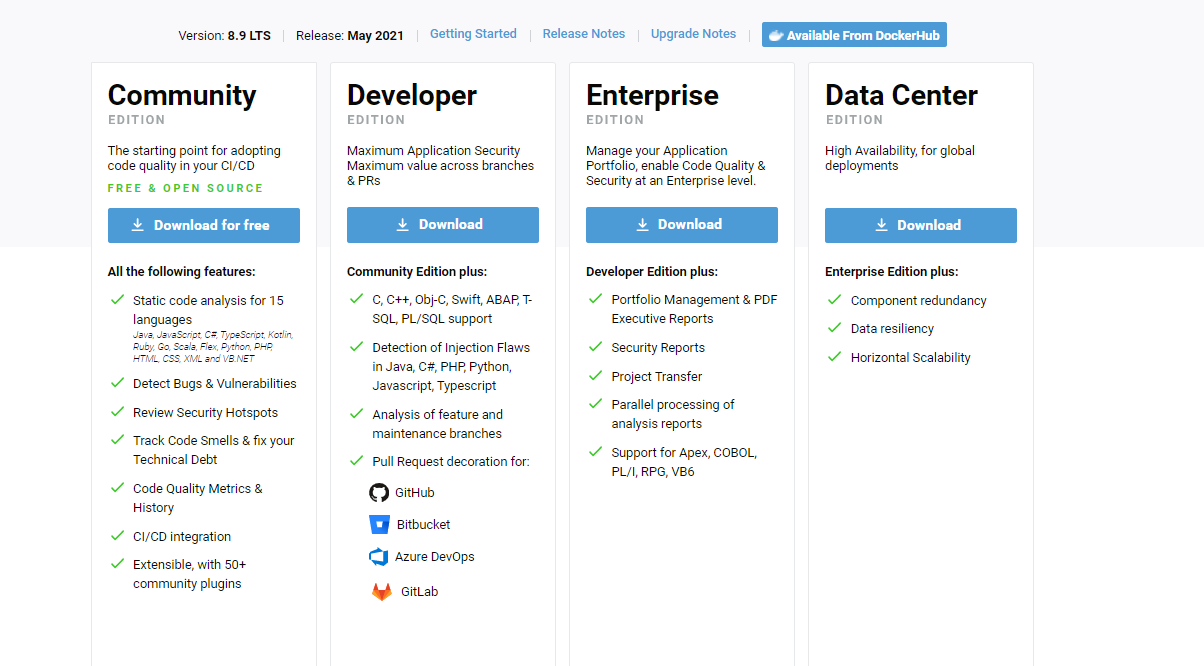
\includegraphics[width=\linewidth]{./imagenes/02_SonarQubeEditions.png}
    \caption{Versiones Sonarqube 8.9.}  
\end{figure}

La versión \emph{“Community”} incluye escáneres para los siguientes lenguajes de programación:

\begin{multicols}{2}
    \begin{itemize}
        \item Java
        \item JavaScript
        \item c\#
        \item TypeScript
        \item Ruby
        \item Go
        \item Scala
        \item Flex 
        \item Python
        \item PHP
        \item HTML 
        \item CSS
        \item XML
        \item VB.Net
    \end{itemize}
\end{multicols}

Además, mediante extensiones de la comunidad podemos añadir escáneres para los siguientes lenguajes:

\begin{itemize}	
    \item PL$\backslash$SQL
    \item C$\backslash$C++
\end{itemize}    
\clearpage
\newpage

\subsubsection{Dependency-check}
Es una herramienta de análisis de dependencias que intenta detectar vulnerabilidades divulgadas públicamente contenidas en las dependencias de 
un proyecto. Para ello, determina si existe un identificador de enumeración de plataforma común (CPE) para una dependencia determinada. Si lo encuentra, generará
un informe vinculado a las entradas \gls{cve} asociadas.

Actualmente OWASP Dependency-Check puede analizar dependencias de proyectos Java y .Net, que se encuentran totalmente soportados otros lenguajes como Ruby, Node.js, 
PHP (composer), Swift Package Manager y Python tienen un soporte más limitado.

El componente de análisis de dependencias de OWASP Dependency-Check puede ser ejecutado de las siguientes formas:

\begin{itemize}
    \item Ant task
    \item \href{https://github.com/jeremylong/DependencyCheck/releases/download/v6.1.6/dependency-check-6.1.6-release.zip}{Command Linet Tool}
    \item Grandle plugin
    \item \href{https://search.maven.org/#artifactdetails%7Corg.owasp%7Cdependency-check-maven%7C6.1.6%7Cmaven-plugin}{Maven plugin}
    \item SBT plugin
\end{itemize}

El uso de dependency-check desde la línea de comandos tiene los siguientes parámetros principales:\\

\begin{table}[!htb]
  \begin{center}
        \begin{tabular}{c| L{12cm}}
        \hline 
        \rowcolor{tema!10}
        \textbf{Parámetro} & \textbf{Descripción}\\
        \hline
        --project & Especifica el nombre del proyecto que aparecerá en el reporte.\\ 
        --scan & Directorio donde se encuentran las librerías de terceros.\\
        --out &  Directorio de salida del reporte de análisis de dependencias.\\
        --suppresion & Fichero .xml que contiene vulnerabilidades que deben de ser excluidas del reporte 
        (falsos positivos)      
    \end{tabular}
    \caption{Parámetros línea comandos dependency-check}
    \label{tab:tabla 1}
\end{center}
\end{table}

Ejemplo de uso:\\
\begin{verbatim}
  dependency-check.bat 
      --project "juice-shop" 
      --scan "D:\CodigoAnalisis\Seguridad\juice-shop\node_modules" 
      --out "D:\CodigoAnalisis\Seguridad\WebGoat.NET\reports" 
\end{verbatim}
\clearpage
\newpage

\subsection{Herramientas de análisis dinámico de código}
Para las ejecuciones de análisis dinámico haremos uso de la herramienta Zed Attack Proxy (ZAP) de OWASP en su versión 2.10. OWASP Zap es una de las herramientas de 
software para análisis dinámico de aplicaciones que es mantenida y distribuida por la organización \href{https://owasp.org/www-project-zap/}{OWASP}. Su principal objetivo es el 
análisis de seguridades en aplicaciones web orientados a empresas, se caracteriza por ser de código abierto y totalmente gratuita.\\

La Interfax de OWASP ZAP Desktop está compuesta de los siguientes elementos:
\begin{figure}[h!] 
    \captionsetup{width=1\linewidth}   
    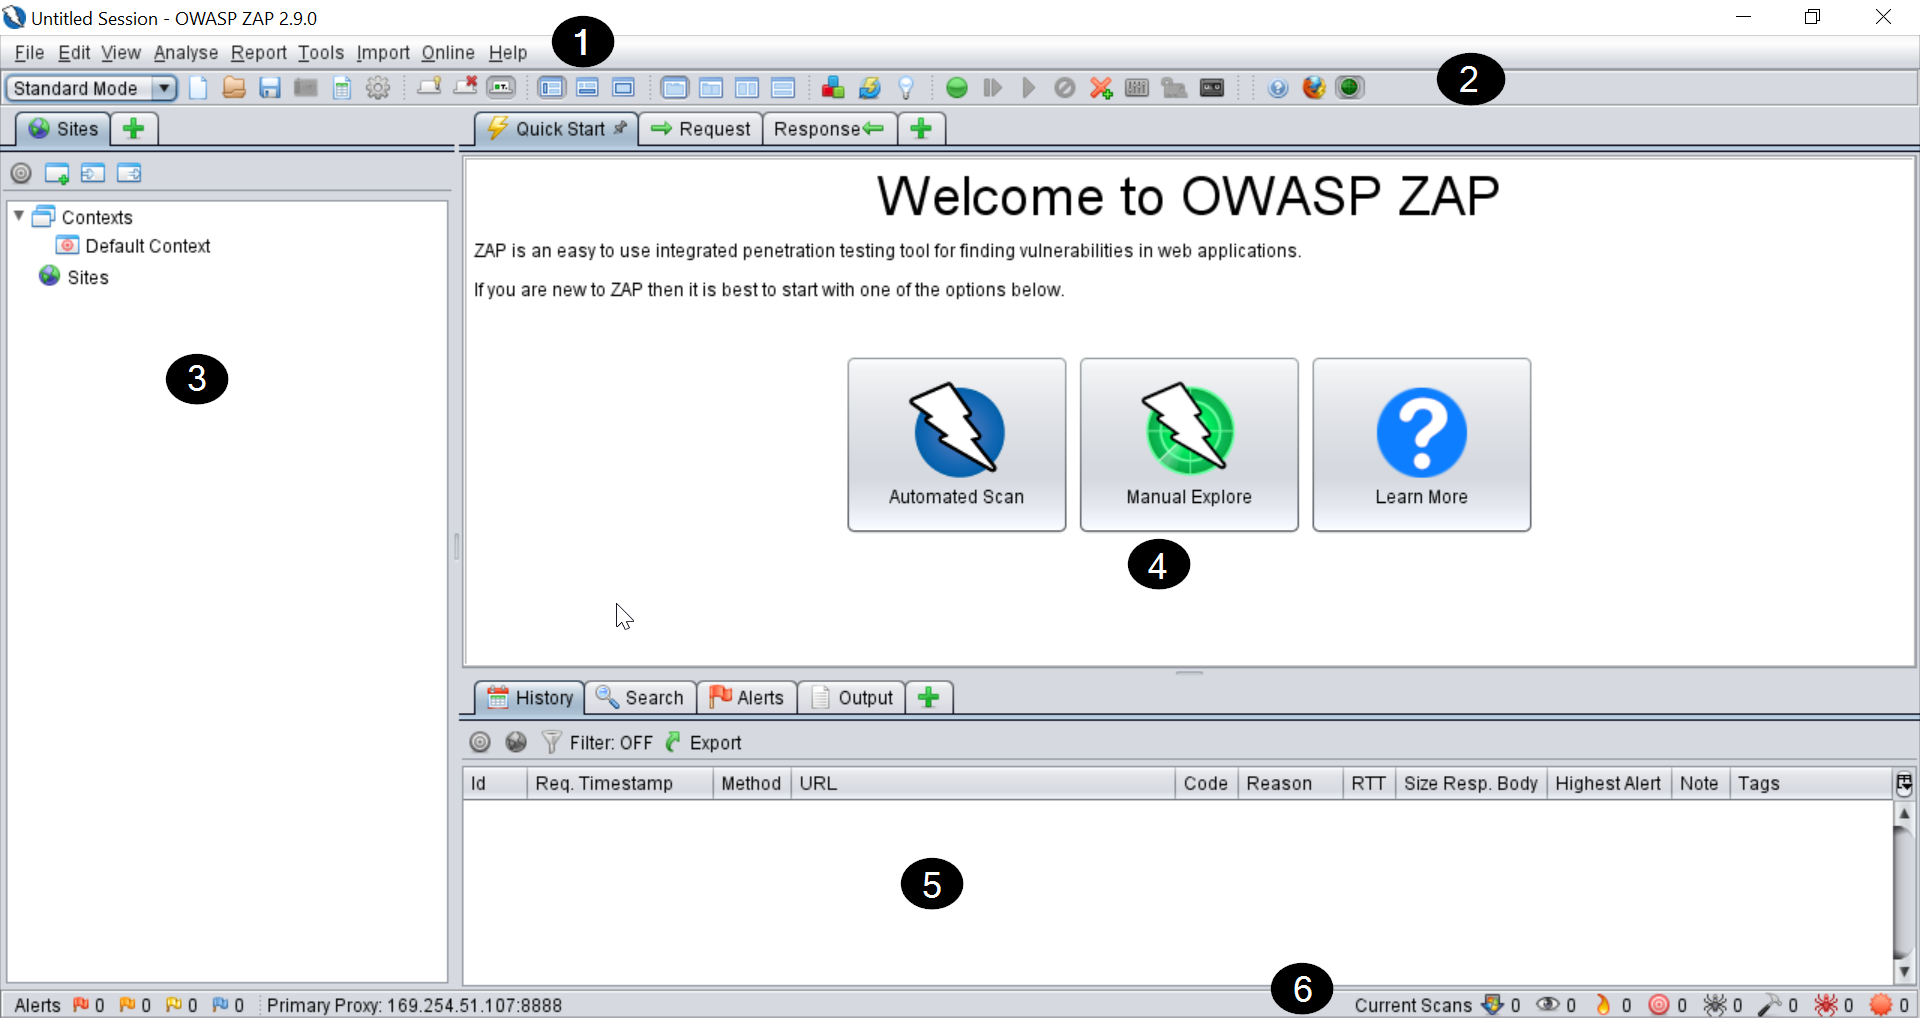
\includegraphics[width=\linewidth]{./imagenes/03_OWASPZAP_Interfaz.png}
    \caption{Interfaz OWASP Zap}  
\end{figure}

\begin{itemize}
    \item \textbf{Barra menú:} Proporciona acceso a las funcionalidades manuales y automáticas de la aplicación.
    \item \textbf{Barra herramientas:} Incluye botones de acceso rápido a las funciones más comunes.
    \item \textbf{Panel vista árbol:} Muestra los sitios visitados, así como los scripts utilizados.
    \item \textbf{espacio de trabajo:} Muestra las peticiones y respuestas de las peticiones y permite editarlas.
    \item \textbf{Ventana de in formación:} Muestra los detalles de las herramientas automáticas y manuales utilizadas. 
    \item \textbf{Pie} Muestra el resumen de alertas encontradas por los distintos escáneres realizados.
\end{itemize}

Para más información consultar documentación, \href{https://www.zaproxy.org/docs/desktop/ui/}{ver documentación ZAP UI}

A la hora de ejecutar el análisis dinámico haremos uso de las siguientes políticas de pruebas 
que serán ejecutados en cada una de las iteraciones para cada aplicación o sistema objetivo:

\begin{itemize}
    \item \textbf{Escáner regular:} Para ampliar las rutas válidas dentro de los dominios a evaluar más allá de la utilizadas en sesión de pruebas utilizada.
    \item \textbf{Escaner Completo:} A partir del resultado del escáner regular, donde se ampliará la batería de pruebas a realizar.
\end{itemize}
